%%%%%%%%%%%%%%%%%%%%%%%%%%%%%%%%%%%%%%%%%
% Masters/Doctoral Thesis 
% LaTeX Template
% Version 2.4 (22/11/16)
%
% This template has been downloaded from:
% http://www.LaTeXTemplates.com
%
% Version 2.x major modifications by:
% Vel (vel@latextemplates.com)
%
% This template is based on a template by:
% Steve Gunn (http://users.ecs.soton.ac.uk/srg/softwaretools/document/templates/)
% Sunil Patel (http://www.sunilpatel.co.uk/thesis-template/)
%
% Template license:
% CC BY-NC-SA 3.0 (http://creativecommons.org/licenses/by-nc-sa/3.0/)
%
%%%%%%%%%%%%%%%%%%%%%%%%%%%%%%%%%%%%%%%%%

%----------------------------------------------------------------------------------------
%	PACKAGES AND OTHER DOCUMENT CONFIGURATIONS
%----------------------------------------------------------------------------------------

\documentclass[
11pt, % The default document font size, options: 10pt, 11pt, 12pt
%oneside, % Two side (alternating margins) for binding by default, uncomment to switch to one side
english, % ngerman for German
singlespacing, % Single line spacing, alternatives: onehalfspacing or doublespacing
%draft, % Uncomment to enable draft mode (no pictures, no links, overfull hboxes indicated)
%nolistspacing, % If the document is onehalfspacing or doublespacing, uncomment this to set spacing in lists to single
%liststotoc, % Uncomment to add the list of figures/tables/etc to the table of contents
%toctotoc, % Uncomment to add the main table of contents to the table of contents
%parskip, % Uncomment to add space between paragraphs
%nohyperref, % Uncomment to not load the hyperref package
headsepline, % Uncomment to get a line under the header
%chapterinoneline, % Uncomment to place the chapter title next to the number on one line
%consistentlayout, % Uncomment to change the layout of the declaration, abstract and acknowledgements pages to match the default layout
]{MastersDoctoralThesis} % The class file specifying the document structure

\usepackage[utf8]{inputenc} % Required for inputting international characters
\usepackage[T1]{fontenc} % Output font encoding for international characters

\usepackage{palatino} % Use the Palatino font by default

\usepackage[backend=bibtex,style=authoryear,natbib=true]{biblatex} % Use the bibtex backend with the authoryear citation style (which resembles APA)

\addbibresource{example.bib} % The filename of the bibliography

\usepackage[autostyle=true]{csquotes} % Required to generate language-dependent quotes in the bibliography

%----------------------------------------------------------------------------------------
%	MARGIN SETTINGS
%----------------------------------------------------------------------------------------

\geometry{
	paper=a4paper, % Change to letterpaper for US letter
	inner=2.5cm, % Inner margin
	outer=3.8cm, % Outer margin
	bindingoffset=.5cm, % Binding offset
	top=1.5cm, % Top margin
	bottom=1.5cm, % Bottom margin
	%showframe, % Uncomment to show how the type block is set on the page
}

%----------------------------------------------------------------------------------------
%	THESIS INFORMATION
%----------------------------------------------------------------------------------------

\thesistitle{Thesis Title} % Your thesis title, this is used in the title and abstract, print it elsewhere with \ttitle
\supervisor{Dr. James \textsc{Smith}} % Your supervisor's name, this is used in the title page, print it elsewhere with \supname
\examiner{} % Your examiner's name, this is not currently used anywhere in the template, print it elsewhere with \examname
\degree{Doctor of Philosophy} % Your degree name, this is used in the title page and abstract, print it elsewhere with \degreename
\author{John \textsc{Smith}} % Your name, this is used in the title page and abstract, print it elsewhere with \authorname
\addresses{} % Your address, this is not currently used anywhere in the template, print it elsewhere with \addressname

\subject{Biological Sciences} % Your subject area, this is not currently used anywhere in the template, print it elsewhere with \subjectname
\keywords{} % Keywords for your thesis, this is not currently used anywhere in the template, print it elsewhere with \keywordnames
\university{\href{http://www.university.com}{University Name}} % Your university's name and URL, this is used in the title page and abstract, print it elsewhere with \univname
\department{\href{http://department.university.com}{Department or School Name}} % Your department's name and URL, this is used in the title page and abstract, print it elsewhere with \deptname
\group{\href{http://researchgroup.university.com}{Research Group Name}} % Your research group's name and URL, this is used in the title page, print it elsewhere with \groupname
\faculty{\href{http://faculty.university.com}{Faculty Name}} % Your faculty's name and URL, this is used in the title page and abstract, print it elsewhere with \facname

\AtBeginDocument{
\hypersetup{pdftitle=\ttitle} % Set the PDF's title to your title
\hypersetup{pdfauthor=\authorname} % Set the PDF's author to your name
\hypersetup{pdfkeywords=\keywordnames} % Set the PDF's keywords to your keywords
}

\begin{document}

\frontmatter % Use roman page numbering style (i, ii, iii, iv...) for the pre-content pages

\pagestyle{plain} % Default to the plain heading style until the thesis style is called for the body content

%----------------------------------------------------------------------------------------
%	TITLE PAGE
%----------------------------------------------------------------------------------------

\begin{titlepage}
\begin{center}

\vspace*{.06\textheight}
{\scshape\LARGE \univname\par}\vspace{1.5cm} % University name
\textsc{\Large Doctoral Thesis}\\[0.5cm] % Thesis type

\HRule \\[0.4cm] % Horizontal line
{\huge \bfseries \ttitle\par}\vspace{0.4cm} % Thesis title
\HRule \\[1.5cm] % Horizontal line
 
\begin{minipage}[t]{0.4\textwidth}
\begin{flushleft} \large
\emph{Author:}\\
\href{http://www.johnsmith.com}{\authorname} % Author name - remove the \href bracket to remove the link
\end{flushleft}
\end{minipage}
\begin{minipage}[t]{0.4\textwidth}
\begin{flushright} \large
\emph{Supervisor:} \\
\href{http://www.jamessmith.com}{\supname} % Supervisor name - remove the \href bracket to remove the link  
\end{flushright}
\end{minipage}\\[3cm]
 
\vfill

\large \textit{A thesis submitted in fulfillment of the requirements\\ for the degree of \degreename}\\[0.3cm] % University requirement text
\textit{in the}\\[0.4cm]
\groupname\\\deptname\\[2cm] % Research group name and department name
 
\vfill

{\large \today}\\[4cm] % Date
%\includegraphics{Logo} % University/department logo - uncomment to place it
 
\vfill
\end{center}
\end{titlepage}

%----------------------------------------------------------------------------------------
%	DECLARATION PAGE
%----------------------------------------------------------------------------------------

\begin{declaration}
\addchaptertocentry{\authorshipname} % Add the declaration to the table of contents
\noindent I, \authorname, declare that this thesis titled, \enquote{\ttitle} and the work presented in it are my own. I confirm that:

\begin{itemize} 
\item This work was done wholly or mainly while in candidature for a research degree at this University.
\item Where any part of this thesis has previously been submitted for a degree or any other qualification at this University or any other institution, this has been clearly stated.
\item Where I have consulted the published work of others, this is always clearly attributed.
\item Where I have quoted from the work of others, the source is always given. With the exception of such quotations, this thesis is entirely my own work.
\item I have acknowledged all main sources of help.
\item Where the thesis is based on work done by myself jointly with others, I have made clear exactly what was done by others and what I have contributed myself.\\
\end{itemize}
 
\noindent Signed:\\
\rule[0.5em]{25em}{0.5pt} % This prints a line for the signature
 
\noindent Date:\\
\rule[0.5em]{25em}{0.5pt} % This prints a line to write the date
\end{declaration}

\cleardoublepage

%----------------------------------------------------------------------------------------
%	QUOTATION PAGE
%----------------------------------------------------------------------------------------

\vspace*{0.2\textheight}

\noindent\enquote{\itshape Thanks to my solid academic training, today I can write hundreds of words on virtually any topic without possessing a shred of information, which is how I got a good job in journalism.}\bigbreak

\hfill Dave Barry

%----------------------------------------------------------------------------------------
%	ABSTRACT PAGE
%----------------------------------------------------------------------------------------

\begin{abstract}
\addchaptertocentry{\abstractname} % Add the abstract to the table of contents
The Thesis Abstract is written here (and usually kept to just this page). The page is kept centered vertically so can expand into the blank space above the title too\ldots
\end{abstract}

%----------------------------------------------------------------------------------------
%	ACKNOWLEDGEMENTS
%----------------------------------------------------------------------------------------

\begin{acknowledgements}
\addchaptertocentry{\acknowledgementname} % Add the acknowledgements to the table of contents
The acknowledgments and the people to thank go here, don't forget to include your project advisor\ldots
\end{acknowledgements}

%----------------------------------------------------------------------------------------
%	LIST OF CONTENTS/FIGURES/TABLES PAGES
%----------------------------------------------------------------------------------------

\tableofcontents % Prints the main table of contents

\listoffigures % Prints the list of figures

\listoftables % Prints the list of tables

%----------------------------------------------------------------------------------------
%	ABBREVIATIONS
%----------------------------------------------------------------------------------------

\begin{abbreviations}{ll} % Include a list of abbreviations (a table of two columns)

\textbf{LAH} & \textbf{L}ist \textbf{A}bbreviations \textbf{H}ere\\
\textbf{WSF} & \textbf{W}hat (it) \textbf{S}tands \textbf{F}or\\

\end{abbreviations}

%----------------------------------------------------------------------------------------
%	PHYSICAL CONSTANTS/OTHER DEFINITIONS
%----------------------------------------------------------------------------------------

\begin{constants}{lr@{${}={}$}l} % The list of physical constants is a three column table

% The \SI{}{} command is provided by the siunitx package, see its documentation for instructions on how to use it

Speed of Light & $c_{0}$ & \SI{2.99792458e8}{\meter\per\second} (exact)\\
%Constant Name & $Symbol$ & $Constant Value$ with units\\

\end{constants}

%----------------------------------------------------------------------------------------
%	SYMBOLS
%----------------------------------------------------------------------------------------

\begin{symbols}{lll} % Include a list of Symbols (a three column table)

$a$ & distance & \si{\meter} \\
$P$ & power & \si{\watt} (\si{\joule\per\second}) \\
%Symbol & Name & Unit \\

\addlinespace % Gap to separate the Roman symbols from the Greek

$\omega$ & angular frequency & \si{\radian} \\

\end{symbols}

%----------------------------------------------------------------------------------------
%	DEDICATION
%----------------------------------------------------------------------------------------

\dedicatory{For/Dedicated to/To my\ldots} 

%----------------------------------------------------------------------------------------
%	THESIS CONTENT - CHAPTERS
%----------------------------------------------------------------------------------------

\mainmatter % Begin numeric (1,2,3...) page numbering

\pagestyle{thesis} % Return the page headers back to the "thesis" style

% Include the chapters of the thesis as separate files from the Chapters folder
% Uncomment the lines as you write the chapters

% Chapter Template

\chapter{Introduction} % Main chapter title

\label{Chapter1} % Change X to a consecutive number; for referencing this chapter elsewhere, use \ref{ChapterX}

%----------------------------------------------------------------------------------------
%	SECTION 1.1
%----------------------------------------------------------------------------------------

\section{Companion Robots}

About companion robots, their purpose.

%-----------------------------------
%	SECTION 1.2
%-----------------------------------
\section{Robot Adaptation in Human Robot Interaction}

About lifelong learning, adaptation and adjustability.

%----------------------------------------------------------------------------------------
%	SECTION 1.3
%----------------------------------------------------------------------------------------


\section{Motivation and Existing Problems}

Sed ullamcorper quam eu nisl interdum at interdum enim egestas. Aliquam placerat justo sed lectus lobortis ut porta nisl porttitor. Vestibulum mi dolor, lacinia molestie gravida at, tempus vitae ligula. Donec eget quam sapien, in viverra eros. Donec pellentesque justo a massa fringilla non vestibulum metus vestibulum. Vestibulum in orci quis felis tempor lacinia. Vivamus ornare ultrices facilisis. Ut hendrerit volutpat vulputate. Morbi condimentum venenatis augue, id porta ipsum vulputate in. Curabitur luctus tempus justo. Vestibulum risus lectus, adipiscing nec condimentum quis, condimentum nec nisl. Aliquam dictum sagittis velit sed iaculis. Morbi tristique augue sit amet nulla pulvinar id facilisis ligula mollis. Nam elit libero, tincidunt ut aliquam at, molestie in quam. Aenean rhoncus vehicula hendrerit.


%----------------------------------------------------------------------------------------
%	SECTION 1.4
%----------------------------------------------------------------------------------------


\section{Major Contributions}

Sed ullamecorper quam eu nisl interdum at interdum enim egestas. Aliquam placerat justo sed lectus lobortis ut porta nisl porttitor. Vestibulum mi dolor, lacinia molestie gravida at, tempus vitae ligula. Donec eget quam sapien, in viverra eros. Donec pellentesque justo a massa fringilla non vestibulum metus vestibulum. Vestibulum in orci quis felis tempor lacinia. Vivamus ornare ultrices facilisis. Ut hendrerit volutpat vulputate. Morbi condimentum venenatis augue, id porta ipsum vulputate in. Curabitur luctus tempus justo. Vestibulum risus lectus, adipiscing nec condimentum quis, condimentum nec nisl. Aliquam dictum sagittis velit sed iaculis. Morbi tristique augue sit amet nulla pulvinar id facilisis ligula mollis. Nam elit libero, tincidunt ut aliquam at, molestie in quam. Aenean rhoncus vehicula hendrerit.

%----------------------------------------------------------------------------------------
%	SECTION 1.4
%----------------------------------------------------------------------------------------


\section{Thesis organization}
%% Chapter Template

\chapter{Theoretical Foundations} % Main chapter title

\label{Chapter2} % Change X to a consecutive number; for referencing this chapter elsewhere, use \ref{ChapterX}

The first step in answering my research question, "How to achieve lifelong learning, adaptation, and adjustability for personalized Human-Robot Interaction?", was to do a research on the Human-Human interaction literature.

In this chapter I will present the theories in which this work is based. This is of great importance in aim of the thesis question in order to integrate different paradigms in a robotic system, which is intended to interact with people in their everyday life.

I will begin by examining the most known Behavior Theories, which have been proposed by the psychology field by many years so far. I then explain the Personality Theories. As there are many models in the literature about personality traits, I chosed the Big Five Personality Trait. I will explain each of these topics, arguing that these theories and model were the most suitable approach to provide answers to my research question. 

After explaining the models of personality, I will describe the Social Cognitive Theory, and how this helped to define the different parts of our framework.

I will follow by briefly explaining the main Emotion Theories, describing the Non-Cognitive Theories and the Cognitive Theories, arguing that the Cognitive approach is more suitable for the purpose of this work. This decision leads to another decision, about the cognitive emotion model to use, I chosed the OCC Model, which I will describe, as well as the reason why I used this specific model.

Also, another topic of vital importance for a system of lifelong learning is the memory system, for which I will mention the diferent kinds of memory that are known. I then will focus on the Episodic Memory to explain how it works and why I used this memory on the proposed framework. 

%----------------------------------------------------------------------------------------
%	SECTION 2.1
%----------------------------------------------------------------------------------------

\section{Behavior Theories}

The aim of this work is to create a framework to achieve a longterm Human-Robot interaction. For this reason, the robot would have to adapt to its users. Nevertheless, the human nature presents differences between one individual to another. Each person has different preferences, then, a robotic behavior that can be seem as a good behavior for one person, can be seen as a bad behavior for another person. 

As social entities, we tend to treat computers and other medias as if they were also social entities, as stated by Reeves and Nass in the Media Equation (\cite{reeves1997media}). In certain ocassions we talk to computers even if they do not understand us. This happens because of our need to communicate in a natural way. This would be accentuated by robots who have a body and can talk to us. Then, if we want to achieve a natural interaction between humans and robots, we should need to base our work on the study of human behavior.

The problem of understanding human behavior have been studied for many years by the field of Psychology. One of the first attempts to explain human behavior was done by Freud, in his the psychoanalysis theory and his studies on the unconscious (\cite{freud1915unconscious}), Freud compare the mind as an iceberg, where in the surface is the conscious mind, below of that is found the preconscious, which are the thoughts that can be retrieved by memory, and finally, the biggest region is the unconscious mind, where are found all our internal desires and primitive wishes, which govern our basic behavior.

Another theory of human behavior, called behaviorism, was developed by John Watson in his article ''Psychology as behaviorist views it" (\cite{watson1913psychology}). This theory, rejects the idea of the consciousness and focus on observable behavior, which can be measureable in an objective way.

Behaviorism was detracted by other researchers, who stated that using experiments with humans creates an artificial environment and low ecological validity, this approach is called Humanistic psychology, which also states that humans can make their own decisions and do not follow a deterministic approach (\cite{rogers1963toward}). 

Gordon Allport was one of the first psychologists who developed a personality trait theory (\cite{allport1937personality}). This approach states that a person can be described by terms called traits. A trait can be seen as a behavior pattern that keeps constant through space and time. The combination of different traits and the different degrees of these, is what gives to an individual an specific personality. I will describe this theory in section \ref{sub:personality-trait-theory}

Other grand theory of human behavior is the Cognitivism theory, also called Social Cognitive Theory, was developed by Albert Bandura (\cite{bandura1989human}), this theory focuses on the mental process of learning and and the dynamic interplay between person, behavior and environment. I will explain this theory in more detail in the section \ref{sub:social-cognitive-theory}.

%----------------------------------------------------------------------------------------
%	SECTION 2.1.1
%----------------------------------------------------------------------------------------

\subsection{Personality Trait Theories}
\label{sub:personality-trait-theory}

We decided to focus on this group of theories because it gives a categorization of different kinds of personalities, and at the same time provides a differentiation between individuals. Also, this has been widely studied before in the field of Human-Computer Interaction (HCI), in order to provide with personality to virtual agents (e.g. \cite{andre2000exploiting}, \cite{allbeck2002toward}, \cite{egges2004generic}). In social robotics, this has been also a topic of interest to provide robots with a personality that best fit with their users (e.g. \cite{woods2005robot}, \cite{tapus2008user}, \cite{hendriks2011robot}).

The personality trait theory has evolved with the pass of the years. I will briefly explain some of the most recognized theories in this domain.

One of the first models of personality traits, is the Gordon Allport’s Trait Theory, this theory classify the traits in three classes: Cardinal traits, Central traits, and Secondary traits. According with this theory, Cardinal traits are the traits that are developed by a person (i.e. kindness, greedy, honesty).  Central traits are seen as common to all people and we have different degrees of them (i.e. friendliness, generosity, anxiety). Secondary traits are considered to be related with attitudes or preferences and only appear under certain situations. The total number of traits was of over 4000.

Eysenck proposed a model of only 3 personality trait (\cite{eysenck1953structure}): Introversion/Extroversion, Neuroticism/Emotional stability, and Psychoticism. This model was critized for using a small sample and only self reporting as source.

Raymond Cattell reducted the number of traits from 4000 to 16 using factor analysis using different sources, he also developed a questionnaire to measure these 16 traits, called the Sixteen Personality Factor Questionnaire (16PF, \cite{cattell1957personality}). 

A model emerged from these previous ones, called The Five Factor Theory of Personality, also called the Big Five personality trait. This model has 5 traits: Extroversion, Neuroticism, Agreeableness, Conscientiousness, and Openness. I will describe this model in more detail in the following section.

%--------------------------------------------------------------------------------------
%	Section
%----------------------------------------------------------------------------------------

\subsubsection{Big Five Personality Trait}

The first researcher who argued the existence of 5 traits of personality was Fiske (\cite{fiske1949consistency}), after that, a number of researchers have converged to the existence of 5 orthogonal factors (\cite{norman1963toward}, \cite{goldberg1993structure}, \cite{digman1996curious}). Even when there is no general concensous on a definitive theory of personality, this theory is the more accepted in the contemporary literature.

Researchers, who defend this theory, state that any reasonable large sample of English trait adjectives will elicit a variant of the Big Five factor structure, and then, all such terms can be represented within this model. It is important to note that each trait can be seen as a dimension, each dimension has to facets, and each facet represent a group of adjectives. An example of the uniqueness of a personality, conformed by the five traits of this model, can be seen in Fig. \ref{fig:big-5-theory}.

\begin{figure}[]
\centering
	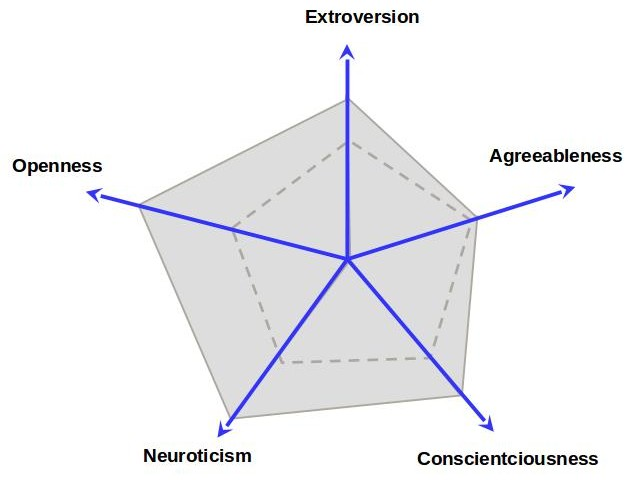
\includegraphics[width=4in]{big-5-theory}
    \caption{Big Five Personality Trait}
\label{fig:big-5-theory}
\end{figure}

This model is also sometimes called OCEAN by the initials of the traits. In the following I will list some of the adjectives grouped on each trait.

\begin{itemize}
\item Openness (Intellect):
	\begin{itemize}
	    \item High Openness: Intellectuallity, depth, insight, intelligence, creativity, curiosity, sophistication.
	    \item Low Openness: Shallowness, unimagitiveness, imperceptiveness, stupidity.
	\end{itemize}
\item Conscientiousness:
	\begin{itemize}
	    \item High Conscientiousness: Organization, efficienty, dependability, precision, persistence, caution, punctuallity, Decisiveness.
	    \item Low Conscientiousness: Desorganization, negligence, inconsistency, forgetfulness, indecisiveness. 
	\end{itemize}
\item Extroversion (Surgency):
	\begin{itemize}
	    \item High Extroversion (Extroversion): Playfulness, expressiveness, spontaneity, talkativeness, animation, courage, optimism.
	    \item Low Extroversion (Introversion): Silence, reserve, shyness, inhibition, passivity, lethargy, pessimism.
	\end{itemize}
\item Agreeableness:
	\begin{itemize}
	    \item High Agreeableness: Cooperation, amability, empathy, generosity, courtesy, flexibility, modesty.
	    \item Low Agreeableness: Belligerence, bossiness, cruelty, pomposity, irritability, prejudice, volatility.
	\end{itemize}
\item Neuroticism (Emotional Stability):
	\begin{itemize}
	    \item High Neuroticism: Insecurity, fear, instability, emotionallity, envy, gullibility, intrusiveness.
	    \item Low Neuroticism: Placidity, independece.
	\end{itemize}
\end{itemize}

A self-reported questionnaire, to measure the five personality traits of this model, was proposed by John and Srivastava, which consited of 44 items in a likert scale from 1-5 (\cite{john1999big}), such questionnaire has been used (or modifications of this) to perform numerous experiments on personality traits in social sciences and also in social robotics.

%----------------------------------------------------------------------------------------
%	SECTION 2.1.2
%----------------------------------------------------------------------------------------

\subsection{Social Cognitive Theory}
\label{sub:social-cognitive-theory}

In the last section, I described the personality traits theories, which explain the differences and similitudes between different individuals. Nevertheless, these theories do not explain how this differences are generated. For this reason, we include a theory that attemps to give a reason of the differences on behaviors between individuals.

This theory sees the human development as a life-long process, where diversity in social practices produces substancial individual differences in the developed capabilities and the ones that remain underdeveloped (\cite{bandura2011social}).

Social Cognitive Theory presents a model of a triadic reciprocal determinism (see Fig. \ref{fig:bandura-theory}), where cognition and other personal factors, behavior, and environment, all influences each other bidirectionally, operating as interacting determinants. This interactions can have different strenghts, and occur in different times. 

\begin{figure}[]
\centering
	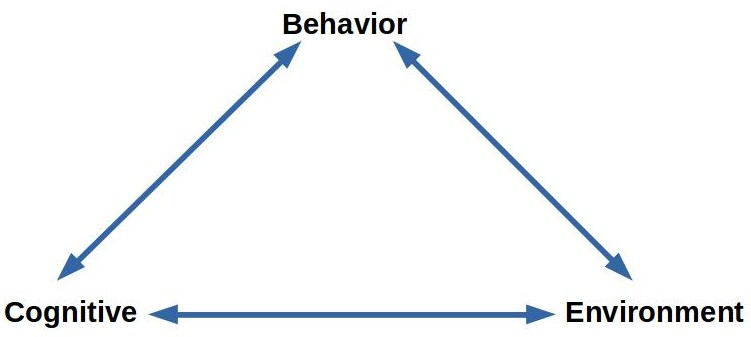
\includegraphics[width=4in]{bandura-theory}
    \caption{Triadic reciprocal determinism}
\label{fig:bandura-theory}
\end{figure}

Persons are characterized in terms of basic capabilities, which are mentioned below:

\begin{itemize}
\item Symbolizing Capability: Humans have the capacity to process external information thanks to the capacity to use symbols. Cognitive factors partly determine in which events we will focus, the related meaning and emotional impact, and how we will organize and use this information on the future.

\item Specialized Cognitive Competencies: Different domains of activity have different structures. Social factors play an influencial role in cognitive development, because of the rapid growth of knowledege, human acquisition of specialized cognitive competencies relies on modeled expertise. 

\item Vicarious Capability (Observational learning): Much social learning occurs by observing the behavior of others and the consequences for them.

\item Forethought capability: People not simply react to their immediate environment, nor are restricted by past experiences. Most human behavior, is regulated by forethought. People motivates themselves and guide their actions anticipatorily.

\item Self-regulatory Capability: Sucessful socialization requires the presence of internal controls and direction. People possess self directive capabilities that give them some control over their thoughts, feelings, and actions.

\item Self-reflective Capability: This capability allow humans to analyze their experiences and to think about their own thought processes. This characteristic acts like a mechanism of adaptation of the thoughts, judging the results of ideas and adequating the thoughts accordingly.

\end{itemize}

This theory, was of great help to integrate the elements of our framework for a robotic system in a social context, even if we don't create specific subsytems for each human capability of the model. For the symbolizing capability, we need a memory system wich also can be combined with the forethought capability, to learn from experiences and adapt the behavior of the robot in future actions. Also an emotion system linked with the memory system is of great importance. The specialized cognitive competences, can be represented by the different task the robot can do, also the information about each user personality and how to act accordingly. 

In the following section I will explain some of the main theories of emotion and the one we used in our framework.


%----------------------------------------------------------------------------------------
%	SECTION 2.2
%----------------------------------------------------------------------------------------

\section{Emotion Theories}

For many years, psychologists have been trying to decide what are the emotions and what are their roles, which remain as open questions until our days. Many theories of emotions has been proposed (For a review, see \cite{moors2009theories}), which can be grouped in two categories: Cognitive theories, and Non-Cognitive theories.
 

%----------------------------------------------------------------------------------------
%	SECTION 2.2.1
%----------------------------------------------------------------------------------------

\subsection{Non-Cognitive Theories  }

This group of theories was first developed by two authors independentely, William James and Carl Lange (\cite{james1884emotion} , \cite{lange1885mechanism}). They stated that an emotional experience is a mental state of bodily response to external stimulus (i.e. "we feel afraid because our body trembles because of a bear"). Williams James considered the emotion as the feeling of the bodily changes that follow the perception of an exciting fact (see Fig.\ref{fig:james-langue}). Lange argued that if we remove of all the bodily sensations, there is nothing left of the emotion, only pure rational knowledge of the event that caused the emotion.

\begin{figure}[]
\centering
	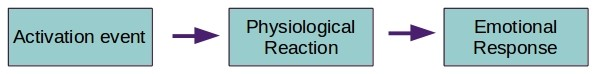
\includegraphics[width=4.6in]{non-cognitive}
    \caption{James-Lange Theory}
\label{fig:james-langue}
\end{figure}

Posteriorly, Paul Ekman developed what is considered the standar of the Non-Cognitive process of emotions. Ekman adopted an evolutionary point of view, where a group of six emotions (happiness, sadness, fear, anger, disgust, and surprise) that he called "basic emotions" (\cite{ekman1992argument}), evolved in response to ecological conditions, and each emotion is linked with a specific neurological circuit. Accordingly to Ekman, the characteristics which distinguis these basic emotions are: Distinctive universal signals, distinctive physiology, quick onset, automatic apraisal, brief duration, unbidden occurrence, distinctive thoughts, and distinctive subjective experience. Also, Ekman stated that each of these basic emotion can be distinguished by different facial expresions (\cite{ekman1979facial}).


%----------------------------------------------------------------------------------------
%	SECTION 2.2.2
%----------------------------------------------------------------------------------------

\subsection{Cognitive Theories }

This group of theories states that emotions are a cognitive process. The precursors of this theories are Walter Cannon and Philip Bard, today known as Cannon-Bard Theory (see Fig.  \ref{fig:cannon-bard}). They stated that we feel emotions and experience physiological reactions at the same time. This theory emerged as a critic of the James-Lange Theory (\cite{cannon1927james}).
Cannon proposed that emotions can be experienced even when physiological reactions are not present, and also that different emotions can present similar reactions (like increasing hearbeat in response to fear or anger).

\begin{figure}[]
\centering
	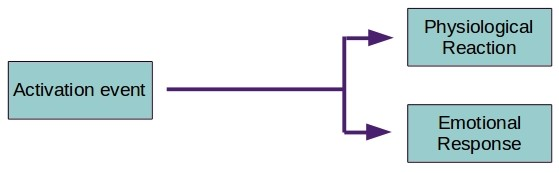
\includegraphics[width=4.6in]{cannon-bard}
    \caption{Cannon-Bard Theory}
\label{fig:cannon-bard}
\end{figure}

Other cognitive theory is the Schachter-Singer Theory (also known as two-factor). This theory proposes that physiological arousal occurs first, but these reactions are often similar to different emotions, then such reactions should be cognitively labeled as a specific emotion (\cite{schachter1962cognitive}).

Richard Lazarus proposed the Cognitive-Mediational Theory (\cite{lazarus1991emotion}), where the appraisal mediates between the stimulus and the emotional response  (see Fig. \ref{fig:lazarus}). This appraisal is the interpretation we give to a particular situation, it can be good or bad, and can be different in different people. Also, Lazarus, distiguish two types of appraisal: 1) primary appraisal, which try to give a meaning to an event, and 2) secondary appraisal, which is the ability to deal with the consequences of an event.

\begin{figure}[]
\centering
	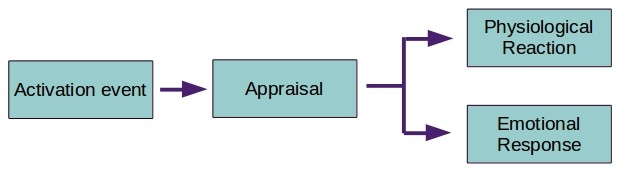
\includegraphics[width=4.6in]{lazarus}
    \caption{Cognitive-Mediational Theory}
\label{fig:lazarus}
\end{figure}

A contemporany theory is the one of Antonio Damasio, called by him the somatic marker hypothesis (\cite{damasio1996somatic}), he states that the emotion process starts with the perception of an stimulus, which provoques a cognitive evaluation, and this generates a bodily response, followed by a perception of a certain body activity (see Fig. \ref{fig:damasio}). Also, Damasio proposes a link between the cognitive evaluation and the perception of activity in the body, called as-if-loop (as if the body were active).

\begin{figure}[]
\centering
	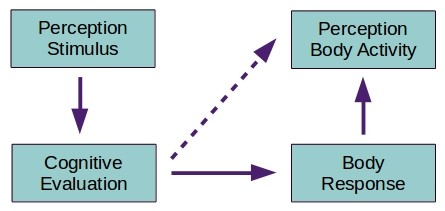
\includegraphics[width=4.6in]{damasio}
    \caption{Damasio's Theory}
\label{fig:damasio}
\end{figure}


%----------------------------------------------------------------------------------------
%	SECTION 2.2.2.1
%----------------------------------------------------------------------------------------

\subsubsection{OCC Model}

%-----------------------------------
%	SECTION 2.3
%-----------------------------------
\section{Learning and Memory}

Nunc posuere quam at lectus tristique eu ultrices augue venenatis. Vestibulum ante ipsum primis in faucibus orci luctus et ultrices posuere cubilia Curae; Aliquam erat volutpat. Vivamus sodales tortor eget quam adipiscing in vulputate ante ullamcorper. Sed eros ante, lacinia et sollicitudin et, aliquam sit amet augue. In hac habitasse platea dictumst.

%----------------------------------------------------------------------------------------
%	SECTION 2.3.1
%----------------------------------------------------------------------------------------

\subsection{Memory Types}

%----------------------------------------------------------------------------------------
%	SECTION 2.3.1.1
%----------------------------------------------------------------------------------------

\subsubsection{Episodic Memory}



%----------------------------------------------------------------------------------------
%	SECTION 3
%----------------------------------------------------------------------------------------

\section{Conclusion}

Sed ullamcorper quam eu nisl interdum at interdum enim egestas. Aliquam placerat justo sed lectus lobortis ut porta nisl porttitor. Vestibulum mi dolor, lacinia molestie gravida at, tempus vitae ligula. Donec eget quam sapien, in viverra eros. Donec pellentesque justo a massa fringilla non vestibulum metus vestibulum. Vestibulum in orci quis felis tempor lacinia. Vivamus ornare ultrices facilisis. Ut hendrerit volutpat vulputate. Morbi condimentum venenatis augue, id porta ipsum vulputate in. Curabitur luctus tempus justo. Vestibulum risus lectus, adipiscing nec condimentum quis, condimentum nec nisl. Aliquam dictum sagittis velit sed iaculis. Morbi tristique augue sit amet nulla pulvinar id facilisis ligula mollis. Nam elit libero, tincidunt ut aliquam at, molestie in quam. Aenean rhoncus vehicula hendrerit.
 
%% Chapter Template

\chapter{State of the Art} % Main chapter title

\label{Chapter3} % Change X to a consecutive number; for referencing this chapter elsewhere, use \ref{ChapterX}

%----------------------------------------------------------------------------------------
%	SECTION 3.1
%----------------------------------------------------------------------------------------

\section{Robots with personality}

Lorem ipsum dolor sit amet, consectetur adipiscing elit. Aliquam ultricies lacinia euismod. Nam tempus risus in dolor rhoncus in interdum enim tincidunt. Donec vel nunc neque. In condimentum ullamcorper quam non consequat. Fusce sagittis tempor feugiat. Fusce magna erat, molestie eu convallis ut, tempus sed arcu. Quisque molestie, ante a tincidunt ullamcorper, sapien enim dignissim lacus, in semper nibh erat lobortis purus. Integer dapibus ligula ac risus convallis pellentesque.

%-----------------------------------
%	SUBSECTION 1
%-----------------------------------
\section{Robots showing emotions}

Nunc posuere quam at lectus tristique eu ultrices augue venenatis. Vestibulum ante ipsum primis in faucibus orci luctus et ultrices posuere cubilia Curae; Aliquam erat volutpat. Vivamus sodales tortor eget quam adipiscing in vulputate ante ullamcorper. Sed eros ante, lacinia et sollicitudin et, aliquam sit amet augue. In hac habitasse platea dictumst.

%-----------------------------------
%	SUBSECTION 2
%-----------------------------------

\section{Robots with Episodic-Memory}
Morbi rutrum odio eget arcu adipiscing sodales. Aenean et purus a est pulvinar pellentesque. Cras in elit neque, quis varius elit. Phasellus fringilla, nibh eu tempus venenatis, dolor elit posuere quam, quis adipiscing urna leo nec orci. Sed nec nulla auctor odio aliquet consequat. Ut nec nulla in ante ullamcorper aliquam at sed dolor. Phasellus fermentum magna in augue gravida cursus. Cras sed pretium lorem. Pellentesque eget ornare odio. Proin accumsan, massa viverra cursus pharetra, ipsum nisi lobortis velit, a malesuada dolor lorem eu neque.

%----------------------------------------------------------------------------------------
%	SECTION 2
%----------------------------------------------------------------------------------------

\section{Conclusion and Horizon}

Sed ullamcorper quam eu nisl interdum at interdum enim egestas. Aliquam placerat justo sed lectus lobortis ut porta nisl porttitor. Vestibulum mi dolor, lacinia molestie gravida at, tempus vitae ligula. Donec eget quam sapien, in viverra eros. Donec pellentesque justo a massa fringilla non vestibulum metus vestibulum. Vestibulum in orci quis felis tempor lacinia. Vivamus ornare ultrices facilisis. Ut hendrerit volutpat vulputate. Morbi condimentum venenatis augue, id porta ipsum vulputate in. Curabitur luctus tempus justo. Vestibulum risus lectus, adipiscing nec condimentum quis, condimentum nec nisl. Aliquam dictum sagittis velit sed iaculis. Morbi tristique augue sit amet nulla pulvinar id facilisis ligula mollis. Nam elit libero, tincidunt ut aliquam at, molestie in quam. Aenean rhoncus vehicula hendrerit.

%% Chapter Template

\chapter{Intregating a Framework for Human-Robot Interaction} % Main chapter title

\label{Chapter4} % Change X to a consecutive number; for referencing this chapter elsewhere, use \ref{ChapterX}

%----------------------------------------------------------------------------------------
%	SECTION 4.1
%----------------------------------------------------------------------------------------

\section{Social Issues of Human-Robot Interaction}

Lorem ipsum dolor sit amet, consectetur adipiscing elit. Aliquam ultricies lacinia euismod. Nam tempus risus in dolor rhoncus in interdum enim tincidunt. Donec vel nunc neque. In condimentum ullamcorper quam non consequat. Fusce sagittis tempor feugiat. Fusce magna erat, molestie eu convallis ut, tempus sed arcu. Quisque molestie, ante a tincidunt ullamcorper, sapien enim dignissim lacus, in semper nibh erat lobortis purus. Integer dapibus ligula ac risus convallis pellentesque.

%----------------------------------------------------------------------------------------
%	SECTION 4.1.1
%----------------------------------------------------------------------------------------

\subsection{Social Facilitation}

Lorem ipsum dolor sit amet, consectetur adipiscing elit. Aliquam ultricies lacinia euismod. Nam tempus risus in dolor rhoncus in interdum enim tincidunt. Donec vel nunc neque. In condimentum ullamcorper quam non consequat. Fusce sagittis tempor feugiat. Fusce magna erat, molestie eu convallis ut, tempus sed arcu. Quisque molestie, ante a tincidunt ullamcorper, sapien enim dignissim lacus, in semper nibh erat lobortis purus. Integer dapibus ligula ac risus convallis pellentesque.

%-----------------------------------
%	SECTION 4.2
%-----------------------------------
\section{Choosing an Emotion Model for the Robot}

Nunc posuere quam at lectus tristique eu ultrices augue venenatis. Vestibulum ante ipsum primis in faucibus orci luctus et ultrices posuere cubilia Curae; Aliquam erat volutpat. Vivamus sodales tortor eget quam adipiscing in vulputate ante ullamcorper. Sed eros ante, lacinia et sollicitudin et, aliquam sit amet augue. In hac habitasse platea dictumst.

%-----------------------------------
%	SECTION 4.3
%-----------------------------------

\section{Giving an Episodic-Memory to the Robot}
Morbi rutrum odio eget arcu adipiscing sodales. Aenean et purus a est pulvinar pellentesque. Cras in elit neque, quis varius elit. Phasellus fringilla, nibh eu tempus venenatis, dolor elit posuere quam, quis adipiscing urna leo nec orci. Sed nec nulla auctor odio aliquet consequat. Ut nec nulla in ante ullamcorper aliquam at sed dolor. Phasellus fermentum magna in augue gravida cursus. Cras sed pretium lorem. Pellentesque eget ornare odio. Proin accumsan, massa viverra cursus pharetra, ipsum nisi lobortis velit, a malesuada dolor lorem eu neque.

%-----------------------------------
%	SECTION 4.4
%-----------------------------------

\section{Testing the Framework in a Game-Like Scenario}
Morbi rutrum odio eget arcu adipiscing sodales. Aenean et purus a est pulvinar pellentesque. Cras in elit neque, quis varius elit. Phasellus fringilla, nibh eu tempus venenatis, dolor elit posuere quam, quis adipiscing urna leo nec orci. Sed nec nulla auctor odio aliquet consequat. Ut nec nulla in ante ullamcorper aliquam at sed dolor. Phasellus fermentum magna in augue gravida cursus. Cras sed pretium lorem. Pellentesque eget ornare odio. Proin accumsan, massa viverra cursus pharetra, ipsum nisi lobortis velit, a malesuada dolor lorem eu neque.

%----------------------------------------------------------------------------------------
%	SECTION 4.5
%----------------------------------------------------------------------------------------

\section{Contributions and Conclusion}

Sed ullamcorper quam eu nisl interdum at interdum enim egestas. Aliquam placerat justo sed lectus lobortis ut porta nisl porttitor. Vestibulum mi dolor, lacinia molestie gravida at, tempus vitae ligula. Donec eget quam sapien, in viverra eros. Donec pellentesque justo a massa fringilla non vestibulum metus vestibulum. Vestibulum in orci quis felis tempor lacinia. Vivamus ornare ultrices facilisis. Ut hendrerit volutpat vulputate. Morbi condimentum venenatis augue, id porta ipsum vulputate in. Curabitur luctus tempus justo. Vestibulum risus lectus, adipiscing nec condimentum quis, condimentum nec nisl. Aliquam dictum sagittis velit sed iaculis. Morbi tristique augue sit amet nulla pulvinar id facilisis ligula mollis. Nam elit libero, tincidunt ut aliquam at, molestie in quam. Aenean rhoncus vehicula hendrerit.
 
%% Chapter Template

\chapter{Need of a User Pattern for a Personalized Interaction} % Main chapter title

\label{Chapter5} % Change X to a consecutive number; for referencing this chapter elsewhere, use \ref{ChapterX}

%----------------------------------------------------------------------------------------
%	SECTION 5.1
%----------------------------------------------------------------------------------------

\section{Choosing a Personality Model}

Lorem ipsum dolor sit amet, consectetur adipiscing elit. Aliquam ultricies lacinia euismod. Nam tempus risus in dolor rhoncus in interdum enim tincidunt. Donec vel nunc neque. In condimentum ullamcorper quam non consequat. Fusce sagittis tempor feugiat. Fusce magna erat, molestie eu convallis ut, tempus sed arcu. Quisque molestie, ante a tincidunt ullamcorper, sapien enim dignissim lacus, in semper nibh erat lobortis purus. Integer dapibus ligula ac risus convallis pellentesque.


%----------------------------------------------------------------------------------------
%	SECTION 5.2
%----------------------------------------------------------------------------------------

\section{Differences between Introverts and Extroverts}

Lorem ipsum dolor sit amet, consectetur adipiscing elit. Aliquam ultricies lacinia euismod. Nam tempus risus in dolor rhoncus in interdum enim tincidunt. Donec vel nunc neque. In condimentum ullamcorper quam non consequat. Fusce sagittis tempor feugiat. Fusce magna erat, molestie eu convallis ut, tempus sed arcu. Quisque molestie, ante a tincidunt ullamcorper, sapien enim dignissim lacus, in semper nibh erat lobortis purus. Integer dapibus ligula ac risus convallis pellentesque.

%-----------------------------------
%	SECTION 5.3
%-----------------------------------
\section{Differences between People with High Conscientiousness and People with Low Conscientiousness}

Nunc posuere quam at lectus tristique eu ultrices augue venenatis. Vestibulum ante ipsum primis in faucibus orci luctus et ultrices posuere cubilia Curae; Aliquam erat volutpat. Vivamus sodales tortor eget quam adipiscing in vulputate ante ullamcorper. Sed eros ante, lacinia et sollicitudin et, aliquam sit amet augue. In hac habitasse platea dictumst.

%-----------------------------------
%	SECTION 5.4
%-----------------------------------

\section{Study-Case: Office-Like Scenario with a Robot Giving Reminders}
Morbi rutrum odio eget arcu adipiscing sodales. Aenean et purus a est pulvinar pellentesque. Cras in elit neque, quis varius elit. Phasellus fringilla, nibh eu tempus venenatis, dolor elit posuere quam, quis adipiscing urna leo nec orci. Sed nec nulla auctor odio aliquet consequat. Ut nec nulla in ante ullamcorper aliquam at sed dolor. Phasellus fermentum magna in augue gravida cursus. Cras sed pretium lorem. Pellentesque eget ornare odio. Proin accumsan, massa viverra cursus pharetra, ipsum nisi lobortis velit, a malesuada dolor lorem eu neque.

%----------------------------------------------------------------------------------------
%	SECTION 5.5
%----------------------------------------------------------------------------------------

\section{Contributions and Conclusion}

Sed ullamcorper quam eu nisl interdum at interdum enim egestas. Aliquam placerat justo sed lectus lobortis ut porta nisl porttitor. Vestibulum mi dolor, lacinia molestie gravida at, tempus vitae ligula. Donec eget quam sapien, in viverra eros. Donec pellentesque justo a massa fringilla non vestibulum metus vestibulum. Vestibulum in orci quis felis tempor lacinia. Vivamus ornare ultrices facilisis. Ut hendrerit volutpat vulputate. Morbi condimentum venenatis augue, id porta ipsum vulputate in. Curabitur luctus tempus justo. Vestibulum risus lectus, adipiscing nec condimentum quis, condimentum nec nisl. Aliquam dictum sagittis velit sed iaculis. Morbi tristique augue sit amet nulla pulvinar id facilisis ligula mollis. Nam elit libero, tincidunt ut aliquam at, molestie in quam. Aenean rhoncus vehicula hendrerit.
 

%----------------------------------------------------------------------------------------
%	THESIS CONTENT - APPENDICES
%----------------------------------------------------------------------------------------

\appendix % Cue to tell LaTeX that the following "chapters" are Appendices

% Include the appendices of the thesis as separate files from the Appendices folder
% Uncomment the lines as you write the Appendices

% Appendix A

\chapter{Evaluation Documents} % Main appendix title

\label{AppendixA} % For referencing this appendix elsewhere, use \ref{AppendixA}

\section{Big Five Questionnaire}

The color of links can be changed to your liking using:

{\small\verb!\hypersetup{urlcolor=red}!}, or

{\small\verb!\hypersetup{citecolor=green}!}, or

{\small\verb!\hypersetup{allcolor=blue}!}.

\noindent If you want to completely hide the links, you can use:

{\small\verb!\hypersetup{allcolors=.}!}, or even better: 

{\small\verb!\hypersetup{hidelinks}!}.

\noindent If you want to have obvious links in the PDF but not the printed text, use:

{\small\verb!\hypersetup{colorlinks=false}!}.

\section{Game-Like Scenario Post-Questionnaire}

The color of links can be changed to your liking using:

\section{Office-Like Scenario Post-Questionnaires}

The color of links can be changed to your liking using:

\section{Multimedia Scenario Post-Questionnaire}

The color of links can be changed to your liking using:

\section{Learning Users' Preferences Post-Questionnaire}

The color of links can be changed to your liking using:
%% Appendix A

\chapter{Publications List} % Main appendix title

\label{AppendixB} % For referencing this appendix elsewhere, use \ref{AppendixB}

%\include{Appendices/AppendixC}

%----------------------------------------------------------------------------------------
%	BIBLIOGRAPHY
%----------------------------------------------------------------------------------------

\printbibliography[heading=bibintoc]

%----------------------------------------------------------------------------------------

\end{document}  
